%
% cmb.tex
%
% (c) 2017 Prof Dr Andreas Müller, Hochschule Rapperswil
%
\chapter{Der kosmische Mikrowellenhintergrund%
\label{skript:chapter:cmb}}
\lhead{Der kosmische Mikrowellenhintergrund}
\rhead{}
Im Kapitel~\ref{skript:chapter:kosmologie} haben wir aus den
Einstein-Gleichungen abgeleitet, dass ein homogenes und isotropes
Universum nicht statisch sein kann.
Hubbles Entdeckung der Expansion des Universums erlaubte uns zu
schliessen, dass das frühe Universum sehr heiss und dicht gewesen
sein muss.
Die Friedmann-Gleichung und ihre ausführliche Diskussion im
Kapitel~\ref{skript:chapter:friedmann} hat gezeigt, wie Materie und
Strahlung im Universum diese Expansion beeinflussen.
Es wurde dort auch auf das Steady-State-Modell hingewiesen, welches
ein sich ausdehnendes Universum konstanter Dichte zulässt.
Dieses wurde mit der Entdeckung des kosmischen Mikrowellenhintergrundes durch
Penzias und Wilson (mehr dazu im Kapitel~\ref{chapter:cmb}) ausgeschlossen.
Es bleibt aber noch zu verstehen, wie der kosmische Mikrowellenhintergrund
entsteht und welche Eigenschaften man von ihm erwarten kann.

Es stellt sich heraus, dass der kosmische Mikrowellenhintergrund mit sehr
hoher Genauigkeit das Spektrum eines schwarzen Körpers hat.
In diesem Kapitel wird daher zunächst ein Überblick über die allgemeine
Theorie der Schwarzkörperstrahlung gegeben.
Im zweiten Abschnitt wird der Ablauf der Rekombination genauer untersucht.
In dieser Phase wird aus dem heissen Plasma ein vergleichsweise kaltes Gas,
in dem sich Licht ungehindert ausbreiten kann.
Die in diesem Moment freigesetzte Strahlung messen wir heute als den
kosmischen Mikrowellenhintergrund.
Im letzten Teil untersuchen wir dann, ob sich mit unserem Wissen
bereits Aussagen über Grösse und Temperatur von Anisotropien im kosmischen
Mikrowellenhintergrund machen lassen.

\section{Thermodynamik und Schwarzkörperstrahlung}
\rhead{Thermodynamik und Schwarzkörperstrahlung}
Ein ungelöstes Problem der Physik im ausgehenden neunzehnten Jahrhundert
war das Strahlungsspektrum eines schwarzen Körpers zu berechnen.
Ein schwarzer Körper ist eine idealisierte thermische Strahlungsquelle,
die auftreffende elektromagnetische Strahlung jeder Wellenlänge absorbiert
und deren Strahlungsspektrum nicht von der Oberflächenbeschaffenheit
abhängt, sondern nur von dessen Temperatur.
Eine mögliche Realisierung ist ein mit Strahlung gefüllter Hohlraum, dessen
Wände auf konstanter Temperatur gehalten werden.

Die klassische Thermodynamik, die im
Abschnitt~\ref{skript:cmb:section:klassisch} zusammengestellt wird,
stellt die Werkzeuge bereit, mit der wir
dem Strahungsgesetz auf den Grund gehen können.
In Abschnitt~\ref{skript:cmb:section:planck} leiten wir daraus
das Plancksche Strahlungsgesetz her.
Insbesondere interessiert uns dabei, dass eine Vergrösserung aller
Wellenlängen um den gleichen Streckungsfaktor die Form des
Strahlungsgesetzes nicht ändert, so dass die Expansion des Universums
die Eigenschaften des Schwarzkörperspektrums erhält.
Daraus werden wir auch ableiten, wie sich die zugehörige Temperatur
mit der Expansion verändert.

%Die kosmische Mikrowellenhintergrundstrahlung wurde in dem Moment
%ausgestrahlt, als das ionisierte Gas frühen Universums neutral wurde,
%man nennt dies die Rekombination.
%Die Dynamik dieses Ereignisses wird in
%Abschnitt~\ref{skript:cmb:section:rekombination} untersucht.

\subsection{Thermodynamik%
\label{skript:cmb:section:klassisch}}
\index{Thermodynamik}%
Ein thermodynamisches System besteht aus einer grossen Zahl von 
Teilchen, die ständig interagieren und dabei Energie austauschen.
Der mikroskopische Zustand des Systems ändert sich laufend
und sehr rasch.
\index{mikroskopischer Zustand}
\index{Zustand, mikroskopisch}
Es ist daher gar nicht möglich, den aktuellen mikroskopischen
Zustand zu beschreiben.
Jede makroskopische Messung liefert daher immer nur einen mittleren
Wert für die gemessene Grösse.

Die fundamentale Zustandsgrösse der klassischen Thermodynamik ist
die Entropie, eine Funktion $S(U,V)$ von inneren Energie $U$ und 
Volumen $V$ des Systems. 
\index{Entropie}%
Alle mikroskopischen Zustände zur gleichen Energie und im gleichen
Volumen sind gleichermassen zulässig.
Offenbar gibt es auch keinen Grund, warum einer dieser Zustände
bevorzugt werden soll.
Die statistische Wärmelehre
{\em postuliert} daher, dass alle mikroskopischen Zustände gleich
wahrscheinlich sind.
Dies bedeutet auch, dass das System immer alle mikroskopischen
Zustände ausnützt, die mit der vorgegebenen inneren Energie $U$ und
dem Volumen $V$ vereinbar sind.
Die Zahl $\Omega(U,V)$ der mikroskopischen Zustände, zwischen denen das
System rasche Übergänge vollführt, nimmt zum Beispiel zu, wenn ein
Ventil geöffnet wird, und dem System damit ein grösseres Volumen
zur Verfügung steht.

Andererseits ist aus der klassichen Thermodynamik bekannt, dass ein
System immer denjenigen Zustand annimmt, in dem die Entropie $S(U,V)$
als Funktion von $U$ und $V$ ihr Maximum annimmt.
Man darf daher schliessen, dass die Entropie als Funktion der Anzahl
$\Omega(U,V)$ der mikroskopischen Zustände ausgedrückt werden kann.
Allerdings ist die Entropie additiv, fügt man zwei Systeme zusammen,
so ist die Entropie des Gesamtsystems die Summe der Entropien der
Teilsysteme:
\[
S(U,V) = S_1(U_1,V_1) + S_2(U_2,V_2).
\]
Die Anzahl der Zustände hingegen ist multiplikativ: da es für jeden
der $\Omega_1(U_1,V_1)$ Zustände des ersten Systems $\Omega_2(U_2,V_2)$
Zustände des zweiten Systems gibt, ist die Gesamtzahl der Zustände
deren Produkt
\[
\Omega(U,V)=\Omega_1(U_1,V_1)\cdot \Omega_2(U_2,V_2).
\]
Die Logarithmus-Funktion erfüllt diese Bedingung, und bis auf einen
Faktor ist sie auch die einzige Funktion mit dieser Eigenschaft.
Man kann also immer
\begin{equation}
S(U,V)=k_B\log \Omega(U,V)
\label{skript:cmb:boltzmann}
\end{equation}
setzen, wobei der Faktor $k_B$ im wesentlichen die Masseinheit von
$S$ festlegt.
Durch die Wahl
\[
k_B = 1.3807\cdot 10^{-23} \text{J}/\text{K}
\]
wird Übereinstimmung mit der Kelvin-Temperaturskala erreicht.
\index{Kelvin-Temperaturskala}%

\subsubsection{Kanonischer Formalismus}
\index{kanonischer Formalismus}%
Dieser Formalismus ist jedoch für die Beschreibung eines Systems 
nicht geeignet, welches sich in Kontakt mit einem Wärmereservoir
befindet, mit welchem es zur Erhaltung der Temperatur Energie
austauschen kann.
Dabei ändert sich die innere Energie des Systems.
Zu dessen Beschreibung ist daher eine Zustandsfunktion nötig, die von
der Temperatur und dem Volumen abhängt, während die Entropie
von innerer Energie und Volumen abhängt.
Man kann dieses Problem lösen, indem man das Wärmereservoir als
Teil eines grösseren Systems modelliert, mit dem das untersuchte
System Energie austauschen kann.
Die Gesamtenergie $E_\text{tot}$ des kombinierten Systems ist dann zwar eine
Zustandsvariable, aber das ursprüngliche Teilsystem kann verschiedene
Zustände annehmen.

Bezeichnen wir die verschiedenen Zustände mit einem Index $j$
und ihre Energie mit $E_j$, dann können wir die Wahrscheinlichkeit
berechnen, dass sich das ursprüngliche System im Zustand $j$ befindet.
Dazu berechnen wir die Anzahl der Zustände, in denen sich das 
Reservoir in einem Zustand mit Energie $E_\text{tot} - E_j$ befindet
und dividieren durch die Gesamtzahl der Zustände mit Energie $E_\text{tot}$.
Wir finden
\[
w_j
=
\frac{\Omega_\text{res}(E_\text{tot}-E_j)}{\Omega_\text{tot}(E_\text{tot})}
\]
für die Wahrscheinlichkeit.
Indem man \eqref{skript:cmb:boltzmann} nach $\Omega$ auflöst, kann $w_j$
durch die Entropie ausgedrückt werden:
\begin{equation}
w_j
=
\frac{\exp\bigl(S_\text{res}(E_\text{tot}-E_j)/k_B\bigr)}{\exp\bigl(S_\text{tot}(E_\text{tot})/k_B\bigr)}
\label{skript:cmb:fj}
\end{equation}
Ist $U$ die mittlere Energie des ursprünglichen Systems im Gleichgewicht,
dann gilt die Additivität der Entropie für das kombinierte System in der Form
\[
S_\text{tot}(E_\text{tot})
=
S(U) + S_\text{res}(E_\text{tot}-U).
\]
Da das Reservoir sehr gross ist, sind die Energien $E_j$ der Zustände des
ursprünglichen Systems im Vergleich zur Gesamtenergie sehr klein,
es ist daher zulässig, die Entropie des Reservoirs linear zu approximieren
\begin{align*}
S_\text{res}(E_\text{tot}-E_j)
&=
S_\text{res}(E_\text{tot}-U+U-E_j)
\\
&=
S_\text{res}(E_\text{tot}-U) + \frac{\partial S_\text{res}}{\partial U}(U-E_j)
\\
&=
S_\text{res}(E_\text{tot}-U) + \frac{U-E_j}{T}
\end{align*}
Setzt man dies in den Ausdruck~\eqref{skript:cmb:fj} für $w_j$ ein, 
erhält man
\[
w_j = e^{(U-TS(U))/k_BT} e^{-E_j/k_BT}.
\]
Man sieht, dass in den Formeln vor allem der Ausdruck $1/k_BT$ vorkommt,
denn man daher mit $\beta=1/k_BT$ abkürzt.
Die Wahrscheinlichkeiten $w_j$ können damit etwas prägnanter als
\begin{equation}
w_j = e^{\beta(U-TS(U))}e^{-\beta E_j}
\label{skript:cmb:fj2}
\end{equation}
geschrieben werden.

\subsubsection{Freie Energie}
Der Ausdruck $F=U-TS(U)$ im Exponenten von~\eqref{skript:cmb:fj2}
heisst die {\em helmholtzsche freie Energie}.
\index{freie Energie}
\index{Energie, freie}
\index{helmholzshe freie Energie}
Die helmholtzsche freie Energie $F$ eines thermodynamischen Systems
gibt an, wieviel Energie bei einem reversiblen, isothermen Prozess zur
Arbeitsleistung zur Verfügung steht. 
Je höher die Temperatur oder die Entropie eines Systems ist, desto geringer
ist die für Arbeitsleistung zur Verfügung stehende freie Energie.
Die freie Energie ist eine Zustandsfunktion der Variablen $T$ und $V$.
Da die Temperatur $T$ als Variable auftritt, eignet sich die freie
Energie als Zustandsfunktion zur Beschreibung eines Systems, welches
sich in Kontakt mit einem Wärmereservoir befindet.

Die Wahrscheinlichkeiten $w_j$ müssen sich zu $1$ summieren, es muss also
gelten
\begin{equation}
1=\sum_{j} w_j = e^{\beta F}\sum_j e^{-\beta E_j}
\qquad
\Rightarrow
\qquad
e^{-\beta F}=\sum_je^{-\beta E_j}=Z.
\label{skript:cmb:Z}
\end{equation}
Die Zahl $Z$ heisst die {\em kanonische Zustandssumme}.
\index{kanonische Zustandssumme}%
\index{Zustandssumme, kanonische}%
Aus ihr kann man die freie Energie berechnen, indem man
\eqref{skript:cmb:Z} nach $F$ auflöst:
\begin{equation}
-\beta F=\log\sum_j e^{-\beta E_j} = \log Z.
\end{equation}
Die Wahrscheinlichkeiten $w_j$ kann man jetzt auch ganz unabhängig vom
Reservoir als
\begin{equation}
w_j
=
\frac{e^{-\beta E_j}}{\sum_j e^{-\beta E_j}}
\end{equation}
ausdrücken.

\subsubsection{Erwartungswert der Energie}
Schliesslich lässt sich auch die mittlere Energie des ursprünglichen
Systems durch $Z$ ausdrücken.
Dazu verwendet man zunächst die Definition 
\[
U
=
\sum_j E_jw_j
=
\frac{1}{\sum_i e^{-\beta E_j}}
\sum_j E_je^{-\beta E_j}
=
\frac1Z \sum_j E_je^{-\beta E_j}
\]
des Erwartungswertes der Energie.
Die Ableitung von $\log Z$ nach $\beta$ liefert aber fast dasselbe:
\begin{align*}
\frac{d}{d\beta} \log Z
&=
\frac1{Z}\frac{dZ}{d\beta}
=
\frac1{Z}\sum_j\frac{de^{-\beta E_j}}{d\beta}
=
-\frac1Z\sum_j E_je^{-\beta E_j}
=
-U,
\end{align*}
die mittlere Energie ist also bis auf ein Vorzeichen auch die Ableitung
von $\log Z$ nach $\beta$.
Damit lässt sich auch die innere Energie
\[
U=-\frac{d}{d\beta}\log Z
\]
des ursprünglichen Teilsystems im Gleichgewicht mit dem Reservoir der
Temperatur $T$ aus der Zustandssumme berechnen.

\subsection{Plancksches Strahlungsgesetz%
\label{skript:cmb:section:planck}}
Die im vorangegangenen Abschnitt zusammengestellten Grundlagen der
statischen Mechanik erlauben uns, das Plancksche Strahlungsgesetz
zu verstehen.
\index{Plancksches Strahlungsgesetz}%
\index{Strahlungsgesetzt von Planck}%

\subsubsection{Frequenzdichte}
Elektromagnetische Strahlung in einem verspiegelten Hohlraum bildet
stehende Wellen,
deren Wellenlänge ein ganzzahliger Bruchteil der Abmessungen des
Hohlraumes sein muss.
Eine solche stehende Welle kann durch einen Vektor
\[
\vec{k} = \begin{pmatrix}k_x\\k_y\\k_z\end{pmatrix}
\]
von ganze Zahlen $k_x,k_y,k_z\in\mathbb Z$ beschrieben werden, der
die Anzahl der Wellenlängen angibt, die in jeder Richtung in die
Abmessungen des Hohlraums hineinpassen.
Sei $L$ die Seitenlänge des Hohlraumes, das Volumen ist dann $V=L^3$.
Eine Welle kann man mit Hilfe der Funktionen
\[
\sin \vec{x}\cdot\vec{k}\frac{2\pi}{L}
\qquad\text{und}\qquad
\cos \vec{x}\cdot\vec{k}\frac{2\pi}{L}
\]
beschreiben.
Der Faktor $2\pi/L$ stellt sicher, dass eine Zunahme einer Koordinate
um $L$ das Argument der Winkelfunktion genau um $2\pi$ vergrössert,
so dass die resultierende Funktion in jeder Koordinate $L$-periodisch ist.

Die Ausbreitungsrichtung einer solchen Welle ist $\vec{k}$.
Die Wellenlänge kann man an einem Vektor $\vec{x}$ ablesen, der
$\vec{x}\cdot\vec{k}=L$ erfüllt, er muss daher die Länge
\[
\lambda
=
|\vec{x}|
=
\frac{L}{|\vec{k}|}
\]
haben.
Die zugehörige Frequenz wird daher
\[
\nu(\vec{k})
=
\frac{c}{\lambda}=|\vec{k}|\frac{c}{L}.
\]

Später wird uns die Anzahl der möglichen Vektoren $\vec{k}$ interessieren,
die auf Frequenzen in einem vorgegeben Intervall $[\nu, \nu+d\nu]$
führen.
Dies ist auch die Anzahl der Vektoren mit ganzzahligen Koordinaten derart,
dass
\[
\frac{L}{c}\nu
\le
|\vec{k}|
\le
\frac{L}{c}(\nu+d\nu)
\]
gilt.
Dies ist aber auch ungefähr das Volumen einer Kugelschale zwischen den
Radien 
\[
r=\frac{L}{c}\nu
\qquad\text{und}\qquad
r+dr=\frac{L}{c}(\nu+d\nu)
\]
Die Volumenformel
\[
V(r)
=
\frac{4}{3}\pi r^3
\]
für eine Kugel vom Radius $r$ liefert für das Volumen
zwischen den beiden Radien
\[
V(r+dr)-V(r)
\simeq
\biggl(\frac{d}{dr} \frac{4}{3}\pi  r^3\biggr) \cdot dr
=
4\pi r^2\,dr.
\]
Daraus liest man ab, dass im Interval $[\nu,\nu+d\nu]$ 
\[
4\pi \frac{L^3}{c^3}\nu^2\,d\nu
=
4\pi \frac{V}{c^3}\nu^2\,d\nu
\]
Frequenzen möglich sind.
Bezogen auf das Volumen $V$ bleibt die Zustandsdichte
\begin{equation}
g(\nu)\,d\nu = \frac{4\pi}{c^3}\nu^2\,d\nu.
\label{skript:cmb:zustandsdichte}
\end{equation}
Allerdings ist zu beachten, dass ein elektromagnetisches Strahlungsfeld
zu jedem Wellenzahlvektor $\vec{k}$ zwei voneinander unabhängige 
Felder mit orthogonalen Polarisierungen ermöglicht, was die Zahl
der Zustände nochmals verdoppelt.

\subsubsection{UV-Katastrophe}
\index{UV-Katastrophe}%
Ein klassischer harmonischer Oszillator kann jede beliebige Energie haben,
da diese nur von der Amplitude abhängt.
Die klassische Thermodynamik leitet aus dem kanonischen Formalismus den
Gleichverteilungssatz ab, der besagt,
dass jeder Freiheitsgrad die gleiche mittlere Energie beiträgt.
Da zu jedem Wellenzahlvektor ein eigener Oszillator und damit ein 
eigener Freiheitsgrad zur Verfügung steht, trägt jeder Wellenzahlvektor
die gleiche Energiemenge bei.
Da es unendlich viele Wellenzahlvektoren gibt, wird die Gesamtenergie
unendlich gross.
Man nennt dies die UV-Katastrophe.
Sie zeigt, dass die klassischen Vorstellungen und insbesondere der
Gleichverteilungssatz nicht anwendbar sind.
Das Problem kann nur gelöst werden, indem man
annimmt, dass die Oszillatoren mit hoher Frequenz nur mit geringerer
Wahrscheinlichkeit angeregt werden.

\subsubsection{Quantenhypothese}
Planck nahm in seiner Verzweiflung an, dass in einem Oszillator mit
Freqeuenz $\nu$ nur die diskreten Vielfachen des Energiequantums $h\nu$ 
erlaubt sind, wobei $h$, das {\em Plancksche Wirkungsquantum}, derart
klein ist, dass es bei hohen Energien gar nicht erst in Erscheinung
tritt.
Der Oszillator mit Frequenz $\nu$ hat daher die Energiezustände
\[
E_j = jh\nu,
\]
und damit die Zustandssumme
\[
Z_\nu
=
\sum_{j=0}^\infty e^{-j\beta h\nu}
=
\sum_{j=0}^\infty \bigl(e^{-\beta h\nu}\bigr)^j.
\]
Dies ist eine geometrische Reihe mit dem Quotienten
$q=e^{-\beta h\nu}$ mit der Summe
\[
Z_\nu
=
\frac1{1-q}=\frac1{1-e^{-\beta h\nu}}.
\]
Die mittlere Energie, die sich im Gleichgewicht in diesem Oszillator 
befindet, ist
\[
E(\nu,T)
=
-\frac{d}{d\beta}\log Z_\nu
=
\frac{h\nu e^{-\beta h \nu}}{1-e^{-\beta h\nu}}
=
\frac{h\nu}{e^{\beta h\nu}-1}
=
\frac{h\nu}{e^{h\nu/k_BT}-1}.
\]

Nun ist aber auch noch zu berücksichtigen, dass nicht jede beliebige
Frequenz möglich ist.
Die Zustandsdichte für die Frequenzen wurde
in~\eqref{skript:cmb:zustandsdichte} bereits bestimmt.
Somit erhalten wir das Plancksche Strahlungsgesetz.
Die im Frequenzinterval $d\nu$ abgestrahlte Energie eines
schwarzen Körpers ist
\begin{equation}
U(\nu,T)\,d\nu
=
2g(\nu)\,d\nu
\frac{h\nu}{e^{h\nu/k_BT}-1}
=
\frac{8\pi}{c^3}\nu^2\,d\nu\frac{h\nu}{e^{h\nu/k_BT-1}}
=
\frac{8\pi h\nu^3}{c^3}\frac{d\nu}{e^{h\nu/k_BT}-1}
\label{skript:cmb:plancknu}
\end{equation}
Der Faktor $2$ rührt von den zwei Polarisierungen her, die die Strahlung
bei gleichem Wellenzahlvektor $\vec{k}$ und damit gleicher Frequenz haben
kann.
Abbildung~\ref{skript:cmb:planckU} zeigt die Abhängigkeit von $U$ von
der Frequenz $\nu$ in doppelt logarithmischer Darstellung.
\begin{figure}
\centering
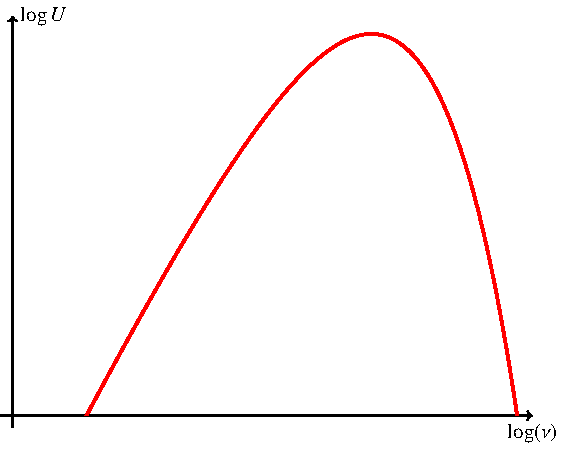
\includegraphics{chapters/tikz/planck1.pdf}
\caption{Plancksches Strahlungsgesetz: Abhängigkeit der Energiedichte
$U(\nu,T)$ von der Frequenz $\nu$ in logarithmischer Darstellung.
\label{skript:cmb:planckU}}
\end{figure}

\subsubsection{Wellenlänge}
\begin{figure}
\centering
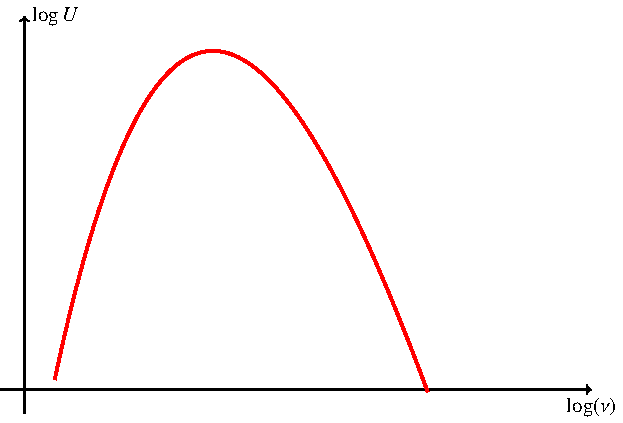
\includegraphics{chapters/tikz/planck2.pdf}
\caption{Plancksches Strahlungsgesetz: Abhängigkeit der Energiedichte
$U(\lambda,T)$ von der Frequenz $\lambda$ in logarithmischer Darstellung.
\label{skript:cmb:planckUlambda}}
\end{figure}
In~\eqref{skript:cmb:plancknu} haben wir das Plancksche Strahlungsgesetz
durch die Frequenz ausgedrückt.
Wir hätten stattdessen auch die Wellenlänge $\lambda=c/\nu$ verwenden 
können.
Einem Interval $[\lambda,\lambda+d\lambda]$ von Wellenlängen entspricht
das Frequenzinterval
\[
\biggl[
\frac{c}{\lambda}-\frac{c}{\lambda^2}d\lambda
,
\frac{c}{\lambda}
\biggr]
\]
und damit das Strahlungsgesetz
\begin{equation}
U(\lambda,T)\,d\lambda
=
\frac{8\pi h}{\lambda^3}\frac{1}{e^{hc/\lambda k_BT}-1}\frac{c}{\lambda^2}\,d\lambda
=
\frac{8\pi hc}{\lambda^5}\frac{1}{e^{hc/\lambda k_BT}-1}\,d\lambda
\label{skript:cmb:planck:lambda}
\end{equation}
in Abhängigkeit von der Wellenlänge $\lambda$ und der Temperatur $T$.
Abbildung~\ref{skript:cmb:planckUlambda} zeigt die Abhängigkeit von
$U(\lambda,T)$ von $\lambda$ in logarithmischer Darstellung.

\subsubsection{Verschiebungsgesetz}
\begin{figure}
\centering
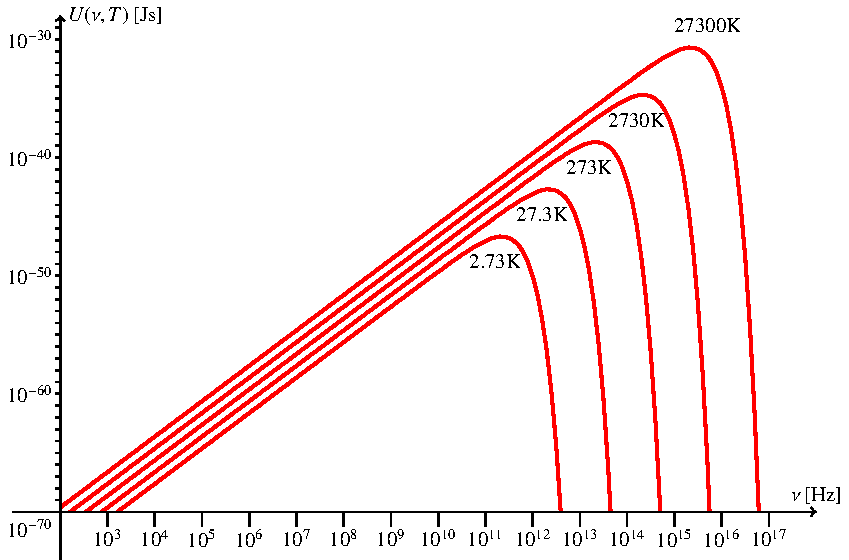
\includegraphics{chapters/tikz/planck3.pdf}
\caption{Abhängigkeit der Schwarzkörperstrahlung von der Temperatur
in doppelt logarithmischer Darstellung.
Man kann gut erkennen, wie das Maximum sich proportional zur Temperatur
verschiebt.
Die unterste Kurve entspricht ungefährt dem Spektrum der Strahlung
des kosmischen Mikrowellenhintergrundes.
\label{skript:cmb:planckverschiebung}}
\end{figure}
Ändert man die Temperatur des Hohlraumes um den Faktor $a$ zur $T_1=aT$,
dann wird sich das Strahlungsspektrum $U_1$ zu anderen Wellenlängen
$\lambda_1$ verschieben.
Wir wollen zeigen, dass mit $\lambda_1=\lambda/a$ wieder ein Plancksches
Strahlungsgesetz entsteht, allerdings mit einer geringeren abgestrahlten
Energie.
Setzen wir dies in das Strahlungsgesetz ein, erhalten wir
\begin{align*}
U_1(\lambda_1,T_1)\,d\lambda_1
&=
B\cdot
U(a\lambda_1,T_1/a)a\,d\lambda_1
\\
&=
\frac{B}{a^4}
\cdot
\frac{8\pi hc}{\lambda_1^5}\frac{1}{e^{hc/\lambda_1k_BT_1}-1}\,d\lambda_1
\\
&=
\frac{B}{a^4}\cdot U(\lambda_1,T_1)\,d\lambda_1.
\end{align*}
Das Strahlungsspektrum bei der Temperatur $T_1=aT$ ist also identisch mit dem
Spektrum bei der Temperatur $T$ mit Wellenlängen, die um den Faktor $a^{-1}$
verkürzt wurden.
Der Faktor $B$ muss $B=a^4$ sein, damit dies zutrifft.
Wir schliessen daraus, dass die Gesamtstrahlung eines schwarzen Körpers
proportional zu $T^4$ sein muss (Wiensches Verschiebungsgesetz).
\index{Wiensches Verschiebungsgesetz}%
\index{Verschiebungsgesetz}%

\subsubsection{Expansion}
In der Form~\eqref{skript:cmb:planck:lambda}
des Strahlungsgesetztes können wir untersuchen was
passiert, wenn sich das ganze Universum, betrachtet als ein gigantischer
Hohlraum, sich um den Faktor $a$ ausdehnt.

Wir bezeichnen die Wellenlänge nach der Expansion mit $\lambda_1=a\lambda$
und bestimmen die Energiedichte $U_1(\lambda_1,T_1)$ in Abhängigkeit von
$\lambda_1$.
Im besten Fall ist $U_1(\lambda_1,T_1)$ wieder das Plancksche
Strahlungsgesetz, möglicherweise mit einer anderen Temperatur $T_1$, die
es ebenfalls zu bestimmen gilt.

Aus dem Strahlungsgesetz~\eqref{skript:cmb:planck:lambda} in Abhängigkeit
von der Wellenlänge wird dann
\begin{align*}
U_1(\lambda_1,T_1)\,d\lambda_1
&=
U(\lambda_1/a,T)\,d(\lambda_1/a)
\\
&=
\frac{8\pi hc}{(\lambda_1/a)^5}
\frac{1}{e^{hc/(\lambda_1/a) k_BT}-1}\,d(\lambda_1/a)
\\
&=
a^4
\frac{8\pi hc}{\lambda_1^5}
\frac{1}{e^{hc/\lambda_1 k_B(T/a)}-1}\,d\lambda_1
\end{align*}
Bis auf den Faktor $a^4$ ist dies wieder ein Plancksches Spektrum
für die Temperatur $T_1=T/a$.
Der Faktor $a^4$ passt aber zu der Tatsache, dass die Gesamtstrahlung
bei einer Temperaturänderung um den Faktor $1/a$ ebenfalls um Faktor
$a^{-4}$ abnehmen muss.
Der Faktor $a^4$ kompensiert also genau diese Abnahme.
Wir kommen daher zum Schluss, dass die Expansion des Universums um den
Faktor $a$ die Temperatur der darin enthaltenen Strahlung um den Faktor
$1/a$ gesenkt wird.
Die Energiedichte der Strahlung nimmt dagegen um den Faktor $a^{-4}$ ab.

\subsubsection{Photonenzahl}
Die Herleitung des Planckschen Strahlungsgesetzes erlaubt auch, die
erwartete Anzahl der angeregten Zustände, also der Photonen im
Hohlraum zu ermitteln.
Wir notieren hier nur das Resultat, die Berechnung findet man zum
Beispiel in \cite[Abschnitt 1.9]{skript:feynman}.
Die Anzahldichte der Photonen in einem Hohlraum der Temperatur $T$ ist
\begin{equation}
n_\gamma
=
16\pi\zeta(3)
\biggl(\frac{k_BT}{hc}\biggr)^3
=
60.422\,
\biggl(\frac{k_BT}{hc}\biggr)^3
=
\frac{16\pi\zeta(3)}{(2\pi)^3}
\biggl(\frac{k_BT}{\hbar c}\biggr)^3
=
0.24359\,
\biggl(\frac{k_BT}{\hbar c}\biggr)^3.
\label{skript:cmb:photonenzahl}
\end{equation}
Darin ist $\zeta(3)$ der Wert der Riemannschen Zetafuntion an der
Stelle $3$.
\index{Riemannsche Zetafunktion}%
\index{Zetafunktion, Riemannsche}%
Ein numerischer Wert ist $\zeta(3)\simeq 1.20205690$.

\section{Entstehung des kosmischen Mikrowellenhintergrundes%
\label{skript:cmb:section:rekombination}}
%\rhead{Entstehung des kosmischen Mikrowellenhintergrundes}
Im frühen Universum war die Energiedichte der Strahlung viel höher
als die Energiedichte der Materie.
Die Friedmann-Gleichung erlaubt den Zeitpunkt zu berechnen,
zu dem die Energiedichte von Strahlung und Materie gleich waren,
wie das in \eqref{skript:friedmann:msequal} durchgeführt wurde.
Im frühen Universum gab es daher einerseits sehr viel mehr Strahlung
als Materie, andererseits war die Dichte höher, so dass es sehr
häufig zu Reaktionen zwischen Atomen und Photonen kam, wodurch die
Atome ionisiert wurden.
Erst als das Universum genügend abgekühlt war, konnten sich Atomkerne
und Elektronen für längere Zeit zusammenfinden.
Man nennt diese Phase die Rekombination, obwohl die Atomkerne und
Elektronen davor noch nie kombiniert gewesen waren.

\rhead{Entstehung des kosmischen Mikrowellenhintergrundes}

In diesem Abschnitt wollen wir daher berechnen, wie der Prozess der
Rekombination abläuft und bei welchem Alter des Universums dies
etwa stattgefunden haben muss.

\subsection{Zusammensetzung des Universums%
\label{section:cmb:dichte}}
Wir nehmen in diesem Abschnitt an, dass das Universum nur aus 
Protonen, Elektronen und Strahlung besteht.
Insbesonderen vernachlässigen wir den beträchtlichen Teil
Helium, der im Rahmen des Big Bang erzeugt worden ist.
Da die Ionisationsenergie von Helium etwa doppelt so hoch ist wie
diejenige von Wasserstoff, muss Helium im wesentlichen bereits
rekombiniert haben in dem Moment, wo die Rekombination des Wasserstoff
stattfindet.
Er hat daher auf den Moment, zu dem das Universum transparent wird
nur geringen Einfluss.

Die Materie im Universum wird beschrieben durch die Anzahldichte
der freien Elektronen $n_e$, die Anzahldichte der freien Protonen $n_p$
und die Anzahldichte $n_\text{H}$ der Wasserstoffatome.
Da das Universum neutral ist, muss $n_e=n_p$ gelten.
Da jedes Wasserstoffatom auch ein Proton als Atomkern enthält, ist die
Gesamtzahl der Baryonen im Universum $n_\text{Baryonen} = n_p+n_\text{H}$.
Sie ist im betrachteten Zeitraum konstant, weil die Temperatur bereits
so tief gesunken ist, dass keine Fusionsprozesse mehr ablaufen können.

Aus Beobachtungen lassen sich Zahlenwerte für diese Anzahldichten abschätzen.
Für die Energiedichte der Protonen wurde ein Wert von
$\varepsilon \simeq 210\,\text{MeV}/\text{m}^3$ gefunden.
Da ein einzelnes Proton die Energie $E_p=939\,\text{MeV}$ hat, finden wir
für die Protonendichte heute
\[
n_{\text{Baryonen}}
=
n_p
\simeq
0.22\,\text{m}^{-3}.
\]
Zum Vergleich: Wasserstoffgas bei Atmosphärendruck hat eine Protonendichte
von etwa $5.3\cdot 10^{25}\,\text{m}^{-3}$.
In einem technischen Ultra-Hochvakuum mit einem Druck von
$10^{-10}\,\text{Pa}$ ist die Protonendichte immer noch
etwa $5.3\cdot 10^{15}\,\text{m}^{-3}$, also über $10$ Grössenordnungen
höher als im Universum im Grossen.

Auch für die Photonendichte kann man eine Schätzung abgeben.
Aus der bekannten Temperatur des kosmischen Mikrowellenhintergrundes
kann man mit der Formel~\eqref{skript:cmb:photonenzahl} die heutige
Photonendichte abschätzen, sie ist
\[
n_{\gamma,0}=4.11\cdot 10^8\,\text{m}^{-3}.
\]
Die Photonendichte ist also auch heute wesentlich höher als die 
Protonendichte, das Verhältnis ist
\[
\eta = \frac{n_{\text{Baryonen}}}{n_\gamma} = 5.35\cdot 10^{-10}.
\]
Die Energie einzelner Photonen der Hintergrundstrahlung ist
allerdings sehr klein.

\subsection{Prozesse in einem vollständig ionisierten Universum}
Wir betrachten das Universum zu einer Zeit, die der Rotverschiebung
$z=10^5$ entspricht.
Das Universum hat damals die Temperatur
$T=zT_0 \simeq 2.725\cdot 10^5\,\text{K}$.
Dies ist zu kalt für Fusionsprozesse, aber die mittlere Energie 
$k_BT\simeq 60\,\text{eV}$ eines Photons ist deutlich höher als die
Ionisationsenergie eines Wasserstoffatoms $Q=13.6\,\text{eV}$,
man kann also davon ausgehen,
dass zu dieser Zeit das Universum vollständig ionisiert war.

Wie gross war die Materiedichte damals? 
Die Materiedichte geht mit der dritten Potenz des Skalenfaktors.
Die Anzahldichte der Baryonen ist daher
\[
n = n_{\text{Baryonen}}(1+z)^3 
\simeq
n_{\text{Baryonen}}\cdot 10^{15}
\simeq
2\cdot 10^{14}\,\text{m}^{-3}.
\]
Dies entspricht einer Massedichte von $3.7\cdot 10^{13}\,\text{kg}/\text{m}^3$,
das war bereits ein extrem verdünntes Plasma.

\subsubsection{Thomson-Streuung}
Der dominierende Prozess in dieser Phase war die {\em Thomson-Streuung}
\[
\gamma + e^- \to \gamma + e^-
\]
\index{Thomson-Streuung}%
eines Photons an einem Elektron.
Diesen Prozess kann man im Labor studieren, er lässt ist durch den
sogenannten Wirkungsquerschnitt
\[
\sigma_e
=
\frac{1}{n_e\lambda}
=
6.65\cdot 10^{-29}\,\text{m}^{-2}
\]
charakterisieren.
Darin ist $n_e$ die Anzahldichte der Elektronen, die mit der Anzahldichte
der Protonen übereinstimmt, und $\lambda$ ist die mittlere freie
Weglänge der Photonen.
Da $n_e$ bekannt ist, kann man dies auch nach $\lambda$ auflösen und
so die mittlere freie Weglänge $\lambda=1/n_e\sigma_e$ finden.
Da sich die Photonen mit Lichtgeschwindigkeit ausbreiten, kann man
die Streurate
\[
\Gamma
=
\frac{c}{\lambda}
=
cn_e\sigma_e\simeq 4.4\cdot 10^{-6}\,\text{s}^{-1}
\]
eines Photons berechnen, das sind etwa 2.6 Streuereignisse pro Woche.
Die Thomson-Streuung tauscht Energie zwischen Photonen und Elektronen aus.
Die Elektronen und die Photonen bilden also ein gekoppeltes thermodynamisches
System.

\subsubsection{Entkoppelung}
Ist die mittlere freie Weglänge grösser als die Hubble-Distanz
(Seite~\pageref{skript:section:hubble-distanz}),
kann ein ``mittleres Photon'' das nächste Streuereignis nicht
mehr erreichen.
Dies tritt ein, wenn $\lambda > c/H$ gilt,
der gleichbedeutend wenn $H>c/\lambda$.
Andererseits ist $\Gamma=c/\lambda$, wir finden daher, dass für 
\[
H>\Gamma
\]
die Streuereignisse verschwinden.

Die Streurate $\Gamma$ nimmt mit der Ausdehnung des Universums ab,
und zwar ist
\[
\Gamma
=
cn_e\sigma_e
\sim
a(t)^{-3}.
\]
Aber auch $H$ nimmt ab,
im Strahlungsdominierten Universum gilt
\[
H^2 = H_0^2  \Omega_{0,s} a(t)^{-4}
\qquad\Rightarrow\qquad
H=H_0\sqrt{\Omega_{0,s}} a(t)^{-2}.
\]
$\Gamma$ nimmt also schneller ab als $H$, es wird also unweigerlich
der Moment eintreten, wo $H>\Gamma$ ist, wo also die Streuprozesse
zum erliegen kommen.
In diesem Moment findet kein bedeutender Energieaustausch mehr statt
zwischen Photonen und Elektronen.
Die Strahlung und die Elektronen entkoppeln.

In dieser Diskussion haben wir aber noch nicht berücksichtigt, dass
die Ausdehnung auch die Temperatur senkt.
Bei niedrigerer Photonenenergie können sich Elektronen und Protonen
zu neutralen Wasserstoffatomen zusammenfinden, man nennt diesen
Prozess die {\em Rekombination}.
\index{Rekombination}%
Fängt ein Proton ein Elektron ein, wird ein Photon ausgesendet,
doch wegen der sehr grossen Zahl der Photonen (dem sehr kleinen Wert
von $\eta$), fallen diese zusätzlichen Photonen nicht ins Gewicht.
Durch die Rekombination werden den Streuprozessen die freien Elektronen
entzogen, der Energieaustausch zwischen Photonen und Elektronen
kommt also bereits früher zum Erliegen.

\subsection{Ionisationsgrad}
Bei der Rekombination nimmt der Anteil des neutralen Wasserstoffs
gegenüber ionisierten Protonen und Elektronen stark zu.
Der {\em Ionisationsgrad} des Universums ist  definiert als
\index{Ionisationsgrad}%
\begin{equation}
X=\frac{n_p}{n_\text{Baryonen}}=\frac{n_p}{n_p+n_\text{H}}.
\label{skript:cmb:Xb}
\end{equation}
Ziel dieses Abschnitts ist, den Prozess der Rekombination besser zu
verstehen durch die Berechnung von $X$ in Abhängigkeit 
von der Zeit.

Löst man die Definition~\eqref{skript:cmb:Xb} nach $n_\text{H}$ auf,
findet man
\begin{align}
\frac1X
&=
\frac{n_p+n_\text{H}}{n_p}
=
1+
\frac{n_\text{H}}{n_p}
\notag
\\
\Rightarrow
\qquad
\frac{n_\text{H}}{n_p}
&=
\frac{1}{X}-1
=
\frac{1-X}{X}
\notag
\\
n_\text{H}
&=
\frac{1-X}{X}n_p.
\label{skript:cmb:XnH}
\end{align}

Ausserdem dürfen wir annehmen, dass die Anzahldichte $n_\gamma$
der Photonen währen der Rekombination wesentlich grösser war als
die Zahl der Baryonen.
Wir bezeichnen mit $\eta$ das Verhältnis
\[
\eta = \frac{n_\text{Baryonen}}{n_\gamma}
\]
von Baryonenzahl zu Photonenzahl.
Mit Hilfe der Definition von $X$ in Gleichung~\eqref{skript:cmb:Xb}
finden wir den Zusammenhang
\begin{equation}
\eta = \frac{n_p}{Xn_\gamma}
\label{skript:cmb:etaX}
\end{equation}
zwischen $\eta$ und $X$.

\subsection{Reaktionsgleichgewicht und Saha-Gleichung}
Die Voraussetzungen über die Zusammensetzung des Universums bedeuten,
dass wir uns nur für die Ionisationsreaktion
\begin{equation}
\text{H} + \gamma 
\rightleftharpoons
p + e^-
\label{skript:cmb:reaktionsgleichung}
\end{equation}
interessieren.
Wir nehmen sogar an, dass die Ionisation eines Wasserstoffatoms 
die konstante Energie $Q=13.6\,\text{eV}$ benötigt.
Damit ignorieren wir angeregt Zustände des Wasserstoffs, die auch
mit geringerem Energieaufwand ionisiert werden können.
Bei der Rekombination ist auch ein Übergang in einen angeregten
Zustand möglich, der später durch Emission eines Photons in den Grundzustand
übergehen kann.

Wir möchten berechnen, wie der Ionisationsgrad sich mit der Zeit ändert.
Wenn die Dichte der Photonen sinkt, wird sich das Reaktionsgleichgewicht
auf die linke Seite von~\eqref{skript:cmb:reaktionsgleichung} verschieben.
Im statistischen Gleichgewicht kann die Maxwell-Boltzmann-Gleichung
verwendet werden, um die Teilchendichte in Abhängigkeit von der Temperatur
auszudrücken, es gilt für die Komponente $x$
\[
n_x
=
g_x \biggl(\frac{m_xk_BT}{2\pi \hbar^2}\biggr)^{\frac32}
\exp\biggl(-\frac{m_xc^2}{k_BT}\biggr).
\]
Die Zahl $g_x$ ist die Anzahl der Zustände mit gleichem Impuls.
Für Elektronen und Protonen ist $g_e=g_p=2$, da beide genau zwei
Spin-Zustände haben.
Das Wasserstoff-Atom hat dagegen $g_\text{H}=4$ Spinzustände.

Das Verhältnis der Anzahldichten der Reaktionsteilnehmer ist
\begin{equation}
\frac{n_\text{H}}{n_pn_e}
=
\underbrace{\frac{g_\text{H}}{g_pg_e}}_{\displaystyle=1}
\biggl(\frac{m_\text{H}}{m_pm_e}\biggr)^{\frac32}
\biggl(\frac{k_BT}{2\pi \hbar^2}\biggr)^{-\frac32}
\exp\biggl( \frac{(m_p+m_e-m_\text{H})c^2}{k_BT} \biggr)
\label{skript:cmb:saha1}
\end{equation}
Mit unseren vereinfachenden Annahmen ist der Zähler im letzten Term
die Ionisationsenergie
\[
Q=(m_p+m_e-m_\text{H})c^2
\]
des Wasserstoffatoms.
Da der Unterschied zwischen $m_p$ und $m_\text{H}$ sehr gering ist,
setzen wir den $m_\text{H}/m_p=1$ im zweiten Faktor auf der rechten Seite
von \eqref{skript:cmb:saha1}.
Mit diesen Vereinfachungen wird die Gleichung~\eqref{skript:cmb:saha1}
zu
\begin{equation}
\frac{n_\text{H}}{n_pn_e}
=
\biggl(\frac{m_ek_BT}{2\pi \hbar^2}\biggr)^{-\frac32}
\exp\biggl( \frac{Q}{k_BT} \biggr),
\label{skript:cmb:saha}
\end{equation}
sie heisst die {\em Saha-Gleichung}.
\index{Saha-Gleichung}%

Man beachte, dass der Faktor
\[
\lambda
=
\sqrt{\frac{2\pi\hbar^2}{m_ek_BT}}
\]
die Dimension einer Länge hat, er heisst auch die thermische de~Broglie
Wellenlänge eines Elektrons mit Temperatur $T$.
Der Faktor vor der Exponentialfunktion in \eqref{skript:cmb:saha}
hat daher die Dimension eines Volumens.

\subsection{Rekombination}
\begin{figure}
\centering
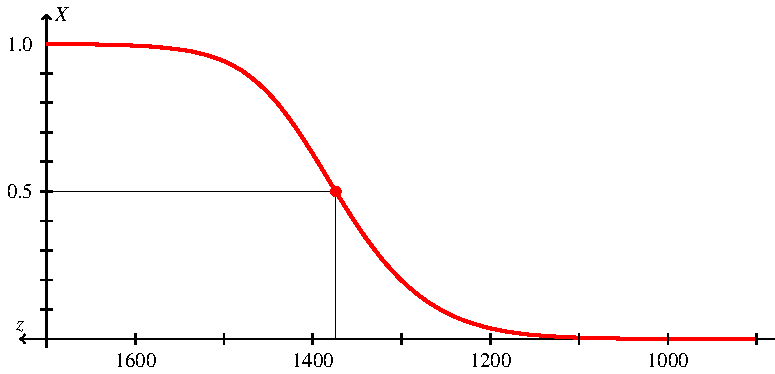
\includegraphics{chapters/tikz/rekombination.pdf}
\caption{Ionisationsgrad in Abhängigkeit von der Rotverschiebung.
Die Zeit läuft von links nach rechts.
Rekombinationszeit ist bei Rotverschiebung $z=1375$ und einer Temperatur
von $T_{\text{rec}}=3747\text{K}$.
\label{skript:cmb:rekombinationgraph}}
\end{figure}
Die Gleichung~\eqref{skript:cmb:XnH} erlaubt uns, in der
Saha-Gleichung~\eqref{skript:cmb:saha} das Verhältnis $m_\text{H}/n_p$
durch $X$ auszudrücken, wir erhalten
\begin{equation}
\frac{1-X}{X}
=
n_p
\biggl(\frac{m_ek_BT}{2\pi \hbar^2}\biggr)^{-\frac32}
\exp\biggl( \frac{Q}{k_BT} \biggr).
\end{equation}
Die Protonendichte $n_p$ lässt sich dank~\eqref{skript:cmb:etaX}
durch $\eta$ und die Photonendichte $n_\gamma$ ausdrücken als
\[
\frac{1-X}{X^2}=\eta n_\gamma
\biggl(\frac{m_ek_BT}{2\pi \hbar^2}\biggr)^{-\frac32}
\exp\biggl( \frac{Q}{k_BT} \biggr).
\]
Für die Hohlraumstrahlung ist die Photonendichte $n_\gamma$ in Abhängigkeit
von der Temperatur aus \eqref{skript:cmb:photonenzahl} bekannt.
\begin{align}
\frac{1-X}{X^2}
&=\eta
\frac{16\pi\zeta(3)}{(2\pi)^3}
\biggl(\frac{k_BT}{\hbar c}\biggr)^3
\biggl(\frac{m_ek_BT}{2\pi \hbar^2}\biggr)^{-\frac32}
\exp\biggl( \frac{Q}{k_BT} \biggr)
\notag
\\
&=
\frac{16\pi\zeta(3)}{(2\pi)^3}(2\pi)^{\frac32}
\,
\eta
\,
\biggl(\frac{k_BT}{m_ec^2}\biggr)^{\frac32}
\exp\biggl( \frac{Q}{k_BT} \biggr)
\\
&=
\frac{16\pi\zeta(3)}{(2\pi)^{\frac32}}
\,
\eta
\,
\biggl(\frac{k_BT}{m_ec^2}\biggr)^{\frac32}
\exp\biggl( \frac{Q}{k_BT} \biggr)
\\
&=
3.8364
\,
\eta
\,
\biggl(\frac{k_BT}{m_ec^2}\biggr)^{\frac32}
\exp\biggl( \frac{Q}{k_BT} \biggr)
\label{skript:cmb:xqauadr}
\end{align}
Schreibt man $S(T,\eta)$ für die rechte Seite von \eqref{skript:cmb:xqauadr},
dann wird daraus eine quadratische Gleichung
\[
1-X-X^2 S(T,\eta)=0
\]
für den Ionisationsgrad, die die Lösungen
\[
X = \frac{-1\pm\sqrt{1+4S}}{2S}
\]
hat.
Nur das positive Zeichen liefert eine positive Lösung, so dass wir
\[
X=\frac{-1+\sqrt{1+4S}}{2S}
\]
erhalten.

\subsubsection{Grendzwerte}
Für $T\to 0$, also für die Zukunft, wird $S\to \infty$ gehen
und damit
\[
\lim_{S\to\infty}\frac{-1+\sqrt{1+4S}}{2S}
=
\lim_{S\to\infty}\frac{1}{\sqrt{S}}
=
0.
\]
Der Ionisationsgrad fällt also in Zukunft gegen 0.

Für $T\to\infty$, also im ganz frühen Universum, geht $S\to 0$
und damit auch $X\to 0$
Hilfe der Regel von de l'H\^opital wird
\begin{align*}
\lim_{S\to 0}\frac{-1+\sqrt{1+4S}}{2S}
&=
\lim_{S\to 0}
\frac{\frac12(1+4S)^{-\frac12} 4S}{2}
=
\lim_{S\to 0}
\frac{\frac12(1+4S)^{-\frac12}\cdot 4}{2}
=
1.
\end{align*}
Im frühen Universum war also das Gas fast vollständig ionisiert.

\subsubsection{Rekombinationszeitpunkt}
Definieren wir willkürlich den Zeitpunkt der Rekombination als
denjenigen Zeitpunkt, zu dem $X=\frac12$ ist, dann gilt auf Grund
von \eqref{skript:cmb:xqauadr}
\[
\frac{1-\frac12}{\bigl(\frac12\bigr)^2}
=
2
=
\frac{16\pi\zeta(3)}{(2\pi)^{\frac32}}
\,
\eta
\,
\biggl(\frac{k_BT_\text{rec}}{m_ec^2}\biggr)^{\frac32}
\exp\biggl( \frac{Q}{k_BT_\text{rec}} \biggr).
\]
Durch Lösung dieser Gleichung\footnote{Im Source-Code Repository findet
man das Octave-Programm \texttt{rekombination.m}, mit dem man die
Funktion $S(T,\eta)$ invertieren kann.}
können wir die Temperatur bestimmen,
bei der die Rekombination stattgefunden hat.
Nimmt man $\eta=5.35\cdot 10^{-10}$, kann man für die Rekombinationstemperatur
\[
T_\text{rec} = 3748\,\text{K}
\]
finden, diese Temperatur tritt ein bei der Rotverschiebung
$z_{\text{rec}} = T_\text{rec}/2.725\,\text{K} -1 = 1374$.
Abbildung \ref{skript:cmb:rekombinationgraph} zeigt den Ionisationsgrad
in Abhängigkeit von der Rotverschiebung.

\subsection{Entkoppelung und letzte Streuung}
Wir können daher die Rotverschiebung genauer ermitteln,
bei der die Entkoppelung stattfinden wird.
Wir wissen bereits, dass dies in dem Moment geschieht, wo
$\Gamma < H$ eintritt.
Die Streurate $\Gamma$ hängt von der Dichte der freien Elektronen
ab, also auch vom Ionsationsgrad, den wir im vorangegangenen Abschnitt
berechnet haben.
Die Abhängigkeit von $H$ von der Rotverschiebung wurde früher schon
bestimmt.

\subsubsection{Ionisationsgrad und Rotverschiebung}
Da wir jetzt den Ionisationsgrad $X$ kennen, kennen wir auch die
Elektronendichte $n_e(z)$ in Abhängigkeit von der Rotverschiebung.
Die Streurate ist
\[
\Gamma(z)
=
n_e(z)\sigma_e c
=
X(z)\cdot n_{\text{Baryonen}} (1+z)^3 \sigma_e c
=
X(z)\cdot 4.4\cdot 10^{-21}\,\text{s}^{-1}.
\]

\subsubsection{Entkopplungszeitpunkt}
Im Materiedominierten Universum gilt
\[
\frac{H^2}{H_0^2}
=
\frac{\Omega_{0,m}}{a_(t)^3}
=
\Omega_{0,m}(1+z)^3
\qquad\Rightarrow\qquad
H
=
H_0\sqrt{\Omega_{0,m}} (1+z)^{\frac32}.
\]
Mit den bekannten Zahlenwerten $\Omega_{0,m}=0.3$ und für $H_0$
findet man
\begin{equation}
H(z)
=
1.202\cdot 10^{-18}\text{s}^{-1} (1+z)^{\frac32}.
\label{skript:cmb:Hz}
\end{equation}
Die Entkopplungsrotverschiebung ist dasjenige $z$, für welches
$\Gamma(z)=H(z)$ gilt, also
\begin{align*}
X(z)\cdot 4.4\cdot 10^{-21} \,\text{s}^{-1}
&=
1.202\cdot 10^{-18}\,\text{s}^{-1} (1+z)^{\frac32}.
\\
1+z_{\text{dec}}
&=
42\cdot X(z_{\text{dec}})^{-\frac23}.
\end{align*}
Löst man diese Gleichung\footnote{Im Repository findet man dazu das
Octave-Programm \texttt{enkoppelung.m}.},
findet man dass die Entkoppelung ungefähr
bei $z_{\text{dec}}=1123$ stattgefunden haben muss.
Genauer
fand dieses Ereignis bei etwa $z=1100$ statt, wie in
\cite[S.~149]{skript:ryden} erklärt wird.
Seit etwa Rotverschiebung $z=1100$ sind die Photonen des kosmischen
Mikrowellenhintergrundes unterwegs, ohne an freien Elektronen gestreut
zu werden.
Man spricht auch von der Fläche der letzten Streuung oder einfach nur
der {\em letzten Streuung}.
\index{letzte Streuung}%

\section{Anisotropie des CMB}
\rhead{Anisotropie des CMB}
Wenige Jahre nach der Entdeckung des kosmischem Mikrowellenhintergrundes
haben verschiedene Experimente versucht, die Vorhersagen zu überprüfen,
die sich aus dem Big-Bang-Modell ableiten lassen:
\begin{enumerate}
\item Die kosmische Hintergrundstrahlung hat das Spektrum eines schwarzen
Körpers.
\item Die kosmische Hintergrundstrahlung ist isotrop.
\end{enumerate}
Im Kapitel~\ref{chapter:cmb} wird etwas detaillierter über die zu diesem
Zweck gestarteten Satellitenmissionen berichtet.
Sie haben Aussage~1 mit grosser Genauigkeit bestätigt und detaillierte
Karten der Anisotropien der Hintegrundstrahlung aufgenommen.
Aussage~2 wurde jedoch nicht exakt bestätigt.
Zwar ist die kosmische Hintergrundstrahlung ausserordentlich isotrop,
es verbleiben aber Anistropien, aus denen sich interessante Schlüsse
über die Frühgeschichte des Universums ziehen lassen.
In diesem Abschnitt soll die Grössse der zu erwartenden Anistropien
abgeschätzt werden.

\subsection{Dipol-Anistropie%
\label{section:cmb:dipolaniso}}
\begin{figure}
\centering
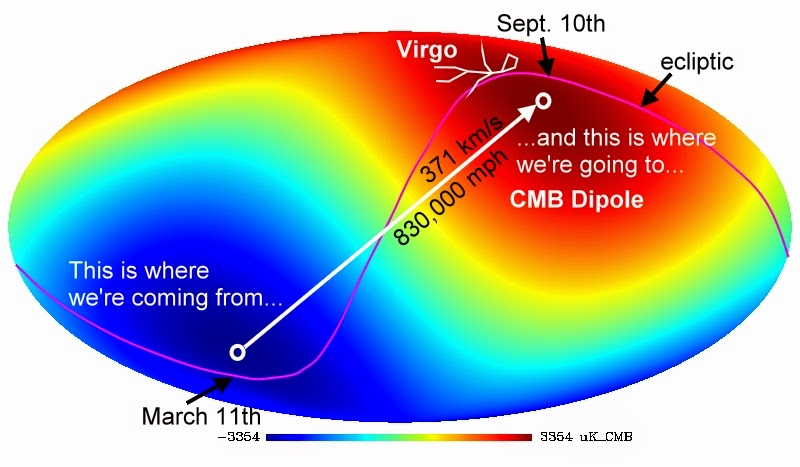
\includegraphics[width=0.8\hsize]{chapters/images/CMBdipole.jpg}
\caption{Dipol-Anistropie des kosmischen Mikrowellenhintergrundes.
\label{skript:cmb:dipolaniso}}
\end{figure}
Der kosmische Mikrowellenhintergrund kommt dem Konzept eines ausgezeichneten
Ruhe-Koor\-di\-na\-ten\-systems am nächsten.
Die Bewegung der Erde um die Sonne, die Bewegung der Sonne um das Zentrum
der Milchstrasse und die Eigenbewegung der Milchstrasse relativ zum
Mikrowellenhintergrund führen dazu, dass die Strahlung aus der Richtung,
in die wir uns bewegen, blauverschoben ist.
Die Strahlung aus der Richtung, aus der wir herkommen, ist dagegen
rotverschoben.

Die Abbildung~\ref{skript:cmb:dipolaniso} zeigt die Dipol-Anistropie, wie
sie von der Planck-Mission gemessen wurde.
\index{Planck-Mission}%
Der gemessene Temperaturunterschied ist $\Delta T= \pm 3.35\,\text{mK}$.
Die zugehörige Geschwindigkeit ist
\[
\frac{\Delta T}{T}=\frac{v}{c}
\qquad\Rightarrow\qquad
v=
\frac{\Delta T}{T}c
=
\frac{3.35\cdot 10^{-3}\,\text{K}}{2.725\,\text{K}}\cdot 2.998\cdot 10^{5}\,\frac{\text{km}}{\text{s}}
=
369\,\frac{\text{km}}{\text{s}}.
\]
Man kann daraus ableiten, dass sich die Erde mit einer Geschwindigkeit von
369\,km/s in Richtung auf das Sternbild Löwe bewegt.

\subsubsection{Höhere Multipole}
\begin{figure}
\centering
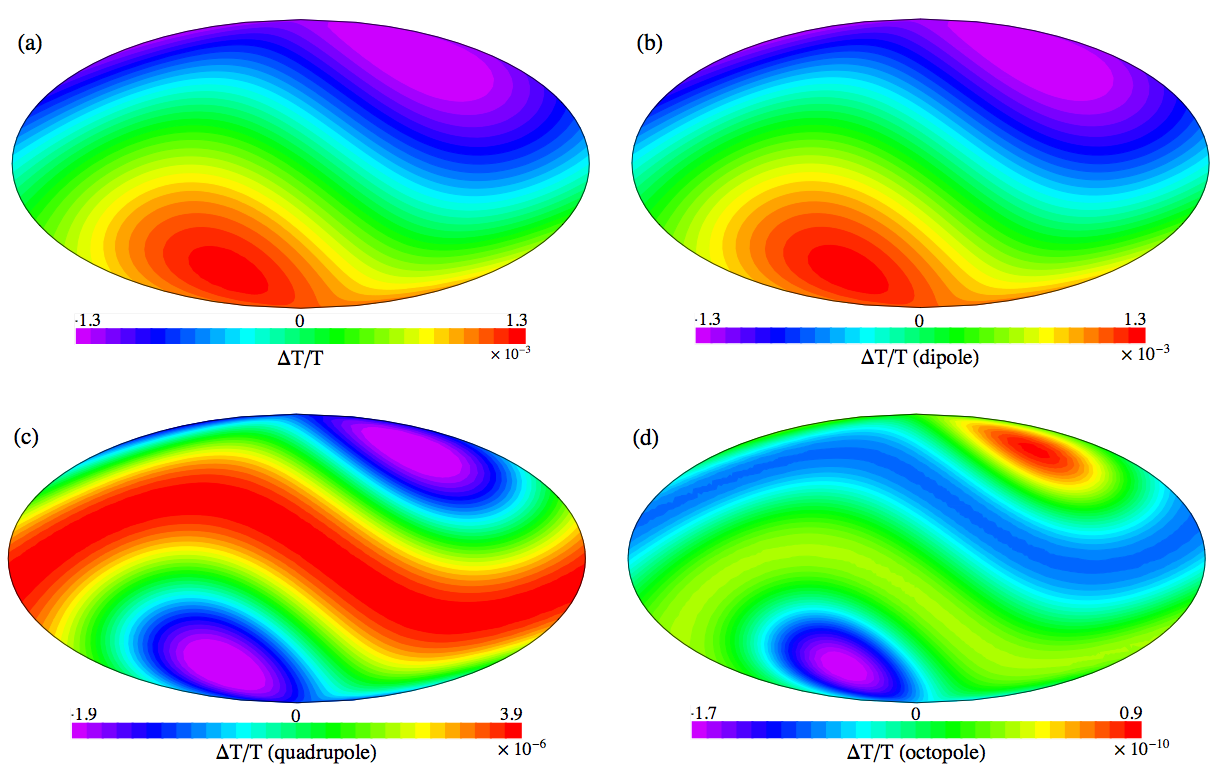
\includegraphics[width=\hsize]{chapters/images/cmb-multipoles.png}
\caption{Multipole der Anistropie des kosmischen Mikrowellenhintergrundes
\cite{skript:cmbmultipoles}.
Die Quadrupol- (c) und Octopol-Anistropien (d) sind mindestens drei
Grössenordnungen geringer als die Dipol-Anistropie (b).
\label{skript:cmb:multipolaniso}}
\end{figure}
Im Kapitel~\ref{skript:chapter:multipol} wurde dargelegt, wie man eine
Funktion auf der Kugeloberfläche nach Kugelfunktionen entwickeln kann.
Die in Abschnitt~\ref{section:cmb:dipolaniso} beschriebene Dipol-Anistropie
entspricht den Termen für $l=1$.
Abbildung~\ref{skript:cmb:multipolaniso} zeigt die nächsthöheren Terme für
$l=2$ und $l=3$ \cite{cmbmultipoles}.
Die Temperatur-Skala verrät, dass diese Anisotropien mindestens drei
Grössenordnungen geringer sind.
Die Dipol-Anistropie ist als bei weitem die dominante Komponente der
Anisotropien des kosmischen Mikrowellenhintergrundes.

\subsection{Hubble-Distanz und Anistropie}
Die maximale Distanz von Punkten, zwischen denen ein Informationsaustausch
möglich ist, ist die Hubble-Distanz
\begin{equation}
l = \frac{c}{H}
\end{equation}
(Abschnitt~\ref{skript:section:hubble-distanz})
\index{Hubble-Distanz}%
Jenseits dieser Distanz ist zum Beispiel kein Temperaturausgleich mehr
möglich, da sogar die Wärmestrahlung als Ausgleichsmechanismus sich zu
langsam ausbreitet.

Die Hubble-Distanz ist für die Kosmologie von besonderer Bedeutung.
Vor der letzten Streuung kann man davon ausgehen, dass die Strahlung
als Temperaturausgleichsmechanismus funktioniert hat und Temperaturdifferenzen
ausgeglichen hat,
die eine kleinere Distanz voneinander entfernt waren als die Hubble Distanz
angibt.
Temperaturdifferenzen, die weiter als eine Hubble-Distanz auseinander lagen
konnten jedoch nicht mehr ausgeglichen werden.
Mit der letzten Streuung entkoppelt sich die Strahlung von der Materie,
jetzt ist es erst recht nicht mehr möglich, dass sich Temperaturunterschiede
ausgleichen können.
Wir erwarten daher, dass wir im kosmischen Mikrowellenhintergrund
Anisotropien von der Grössenordnung der Hubble-Distanz zur Zeit der
letzten Streuung beobachten können.

Seit der letzten Streuung ist das Universum von Materie dominiert,
wir können daher die ungefähre Grösse der Hubble-Konstante zur
Zeit der letzten Streuung mit Hilfe der
Friedmann-Gleichung \eqref{skript:friedmann:omegagleichung}
abschätzen.
Zunächst ist
\[
H(t) = H_0\sqrt{\Omega_{0,m}}\frac{1}{a(t)^\frac32},
\]
wobei wir für die beiden Konstanten $H_0$ und $\Omega_{0,m}$ die
im Standardmodell üblichen Werte
\[
H_0
=
67.74\,\frac{\text{km/s}}{\text{Mpc}}
\qquad\text{und}\qquad
\Omega_{0,m}=0.3
\]
wählen.
Die letzte Streuung erfolgt bei einer Rotverschiebung von $z=1100$, also
gilt
\[
H(t_{\text{ls}})
=
H_0\sqrt{\Omega_{0,m}}\frac{1}{a(t_{\text{ls}})^\frac32}
=
H_0\sqrt{\Omega_{0,m}}(1+z)^\frac32.
\]
Setzen wir die genannten Zahlenwerte ein, erhalten wir
\[
H(t_{\text{ls}})
=
67.74\cdot \sqrt{0.3}\cdot 1101^\frac32
=
1.355\cdot 10^{6}\,\frac{\text{km/s}}{\text{Mpc}}
\]
für die Hubble-Konstante und 
\[
d
=
\frac{c}{H(t_{\text{ls}})}
=
\frac{2.998\cdot 10^{5}\,\text{km/s}}%
{1.355\cdot 10^{6}\,\frac{\text{km/s}}{\text{Mpc}}}
=
0.221\,\text{Mpc}
\]
für die Hubble-Distanz zur Zeit der letzten Streuung.
Zum Vergleich: unsere Milchstrasse hat einen maximalen Durchmesser
von etwa 55\,kpc, die Andromeda-Galaxie ist etwa 770\,kpc entfernt.
\index{Andromeda-Galaxie}%
Die Hubbledistanz zur Zeit der letzten Streuung ist als etwa viermal
so gross wie der Durchmesser der Milchstrasse und etwa ein Viertel der
Entfernung zur Andromeda-Galaxie.
Die im kosmischen Mikrowellenhintergrund sichtbaren Anisotropien
entsprechen daher Strukturen von der grösse des lokalen Haufens von
Galaxien.
\index{lokale Gruppe}%
Inzwischen sind diese jedoch angewachsen auf Strukturen von über 200\,Mpc,
dies entspricht etwa der Grössenordnung der Supercluster.
Dar Laniakea-Supercluster, dem unsere Milchstrasse angehört, hat zum Beispiel
eine Länge von 153\,Mpc.
\index{Laniakea-Supercluster}%
\index{Supercluster}

\subsection{Horizont-Distanz}
Wie weit weg sind die Anisotropien des kosmischen Mikrowellenhintergrundes,
die wir heute beobachten?
Oder allgemeiner: wie weit ist die Quelle eines Photons heute von uns
entfernt, welches bei einer Rotverschiebung $z$ ausgesandt wurde?
Die gesuchte Distanz heisst die {\em Horizont-Distanz}.
\index{Horizont-Distanz}

Nehmen wir also an, ein Photon sei zur Zeit $t$ ausgestrahlt worden,
es war also während der Zeit $t_0-t$ mit Lichtgeschwindigkeit unterwegs,
und hat daher die Distanz $c(t_0-t)$ zurückgelegt.
Wir teilen jetzt des Zeitinterval zwischen $t$ und $t_0$ in kleine
Intervalle der Länge $dt$.
Das Photon legt während dieser Zeit die Distanz $c\,dt$ zurück.
Jedes solche Interval ist seither auf
\[
\frac{a(t_0)}{a(t)}\cdot c \,dt
\]
angewachsen.
Die gesamte Distanz zwischen zur Quelle ist daher
\begin{equation}
d_\text{hor} = c \int_t^{t_0} \frac{a(t_0)}{a(t)}\,dt.
\label{skript:cmb:horizontallg}
\end{equation}

\subsubsection{Skalenfaktor im materiedominierten Universum}
Für die Zeit seit der letzten Streuung lässt sich $a(t)$ als
Lösung der Friedmann-Gleichung eines materiedominierten
Universums finden.
Die zu lösende Differentialgleichung ist
\[
\frac{\dot a(t)^2}{a(t)^2}
=
H_0^2\Omega_{0,m}\frac1{a(t)^3},
\]
die wir nach $\dot a(t)$ auflösen können:
\[
\dot a(t)
=
H_0\sqrt{\Omega_{0,m}} a(t)^{-\frac12}.
\]
Diese Differentialgleichung hat die Lösung
\begin{equation}
a(t) = \biggl(\frac{t}{t_0}\biggr)^\frac23.
\label{skript:cmb:skalenfaktormaterie}
\end{equation}

\subsubsection{Horizontdistanz im materiedominierten Universum}
Aus
\eqref{skript:cmb:horizontallg}
und
\eqref{skript:cmb:skalenfaktormaterie}
lässt sich jetzt die Horizont-Distanz für jede beliebige 
Rotverschiebung berechnen.
Es ist folgt durch Einsetzen von
\eqref{skript:cmb:skalenfaktormaterie}
in
\eqref{skript:cmb:horizontallg}
nämlich
\begin{align*}
d_{\text{hor}}(t)
&=
c\int_t^{t_0} \frac{dt}{(\tau/t_0)^\frac23}
=
3ct_0\biggl(1-\biggl(\frac{t}{t_0}\biggr)^\frac13\biggr)
=
3ct_0(1-a(t)^\frac12)
\end{align*}
Für ein solches Universum gilt aber nach
\eqref{skript:section:hubble-distanz}
auch 
\[
t_0=\frac{2}{3H_0},
\]
so, dass die Horizontdistanz in Abhängigkeit von der Rotverschiebung $z$
\[
d_{\text{hor}}(t)
=
3ct_0\biggl(1-\frac1{\sqrt{1+z}}\biggr)
=
2\frac{c}{H_0}(1-a(t)^\frac12)
=
\frac{2c}{H_0}\biggl(1-\frac{1}{\sqrt{1+z}}\biggr)
\]
ist.
Für die Rotverschiebung der letzten Streuung von $z=1100$ folgt, dass
die Horizontdistanz
\[
d_{\text{hor}}(t_{\text{ls}})
=
3ct_0 \biggl(1-\frac{1}{\sqrt{1101}}\biggr)
=
2.90958 ct_0
\]
ist.
Die Fläche der letzten Streuung ist also fast drei mal so weit von uns
entfernt wie ein Photon seit dem Big Bang unterwegs sein konnte.
Setzt man $t_0=13.7$\,Jahre ein, findet man eine Entfernung von ungefähr 
12\,200\,Mpc.
Eine genauere Rechnung unter berücksichtigung der anderen Komponenten
des Universums, insbesondere der dunklen Energie führt auf die
aktuelle Horizont-Distanz von etwa 14\,000\,Mpc.

\subsection{Anisotropien des CMB}
Die Anistropien des kosmischen Mikrowellenhintergrundes waren
bei ihrer Entstehung von der Grössenordung der der Hubble-Distanz zur
Zeit der letzten Streuung, also
\[
\frac{c}{H(z_{\text{ls}})}
\simeq
0.221\,\text{Mpc},
\]
wie man aus \eqref{skript:cmb:Hz} berechnen kann.

Wenn wir die Anistropien beobachten, müssen wir berücksichtigen, dass
die Strahlung schon sehr lange unterwegs ist.
Die aktuelle Horizontdistanz ist 14\,000\,Mpc, doch zur Zeit der
letzten Streuung bei $z=1100$ war diese Distanz $1100$-mal kleiner,
also nur etwa 13\,Mpc.
Die Anistropien im kosmischen Mikrowellenhintergrund erscheinen uns
daher unter dem Winkel
\[
\frac{0.221\,\text{Mpc}}{13\,\text{Mpc}}
=
0.017
=
0.974^\circ.
\]
Auf einem halben Umfang der Himmelskugel haben daher etwa
\[
l=180^\circ\!/0.974^\circ = 184
\]
solche Anistropien Platz.
Wir erwarten daher, dass bei der Analyse des kosmischen
Mikrowellenhintergrundes mit Kugelfunktionen bei $l\simeq 200$
ein Maximum auftreten wird.
Dies wird im Kapitel~\ref{chapter:cmb} aufs schönste bestätigt.

Für eine Diskussion der physikalischen Gründe, warum die Hubble-Distanz
zur Zeit der letzten Streuung tatsächlich die richtige Grössenordnung
für die Anistropien ist,
siehe \cite{skript:ryden}.




